\section{Analiza wymagań}
\subsection{Opis problemu}
\begin{par}
	Tematem pracy jest zaprojektowanie i implementacja systemu podejmującego decyzje w prostej grze platformowej czasu rzeczywistego.
	Moduł odpowiedzialny za optymalizację przejścia gry, oraz podejmowanie akcji powinien być oparty o zagadnienie algorytmów genetycznych.
	Celem samej gry jest dotarcie do zdefiniowanego wcześniej celu na mapie. Wynik końcowy przejścia może zależeć od wielu parametrów - mapa może zawierać elementy dające punkty, jak i elementy prowadzące do natychmiastowego zakończenia gry (z wynikiem pozytywnym bądź negatywnym).
	Efektem pracy powinien być system pozwalający na rozwiązanie tego typu problemu bazujący na algorytmie genetycznym.
	\newline
	Ogólne wymogi dotyczące systemu:
	\begin{itemize}
		\item
			System powinien składać się z bazowego silnika gry, wzorowanego na rozwiązaniach w klasycznych grach platformowych. Ma to być jednocześnie warstwa prezentacyjna algorytmu.
		\item
			System powinien pozwalać zarówno na poruszanie się po mapie przez użytkownika jak i przejście w tryb treningu populacji, który na podstawie zadanych parametrów optymalizuje przejście po mapie algorytmem genetycznym.
		\item
			Do wyniku końcowego mogą być brane pod uwagę również inne zdarzenia takie jak ilość zebranych obiektów na planszy, czy czas przejścia mapy.
			Funkcja przystosowania zależeć będzie od rożnych czynników, a ustawienie odpowiednich wag może nakierować algorytm na określoną ścieżkę rozwoju.
		\item
			Praca ma mieć charakter edukacyjno-badawczy. Przydatnymi narzędziami w systemie będzie prosty w obsłudze edytor map, panel konfiguracyjny w którym możemy edytować większość parametrów związanych z samym działaniem algorytmu oraz aktywny podgląd populacji i osobników.
	\end{itemize}
\end{par}

\begin{par}
	Sam pomysł stworzenia sztucznej inteligencji do gry platformowej w czasie rzeczywistym został już wcześniej powoływany do życia, m.in. jako projekt MarioAI. 
	W chwili obecnej funkcjonuje on jako turniej dla programistów. 
	Uczestnicy mogą implementować własne rozwiazania do gotowego silnika generującego losowe poziomy, oraz porównywać wyniki z innymi uczestnikami.
	Samo zgłoszenie składa się z implementacji własnej klasy odpowiedzialnej za podejmowanie decyzji.
	Strona domowa projektu znajduje się pod adresem www.marioai.org.
\end{par}



\subsection{Wstępna analiza problemu}
\begin{par}
	Aby dobrze zrealizować część odpowiedzialną za sterowanie postacią, należy użyć klasy pośredniej pomiędzy warstwą logiki silnika gry, a warstwą komunikacji z graczem. 
	Wówczas możemy łatwo zmienić źródło sygnałów wysyłanych do postaci z bezpośrednich zdarzeń z klawiatury na akcje przechowywane przez chromosom. 
	\subsubsection{Projekt chromosomu}
	Kolejnym ważnym elementem jest odpowiednie zaprojektowanie struktury chromosomu. 
	Dwa najbardziej trafne rozwiązania opierają się na dwóch zmiennych występujących w środowisku gry:
	\begin{enumerate}
	\item
	{\bf Czas który upłynął od rozpoczęcia danej instancji przejścia. }
	\begin{par}

		To rozwiązanie zakłada podejmowanie akcji w oparciu o aktualy czas w grze, a sama tablica akcji przechowuje akcje których wykonanie następowałoby po kolei z pewnym interwałem, np. 30 ms (co daje ok 33 akcje w ciągu sekundy).
		Warto zauważyć że dzięki temu iż przebieg symulacji nie zależy od pozycji gracza, mamy swobodę ruchu, a jeśli to korzystne możemy założyć iż dobrym rozwiązaniem w niektórych przypadkach będzie np. odczekanie określonego czasu, bądź powrót do miejsca w którym już byliśmy.
		Istotną wadą tego rozwiązania była duża podatność algorytmu na zapętlanie się, lub wykonywanie dużej ilości mało przydatnych ruchów. 
		Jeśli chcielibyśmy dobrze zaprojektować taki algorytm musielibyśmy brać pod uwagę fakt, iż średnio przy równym prawdopodobieństwie ruchu w lewo jak i prawo, postać będzie przesuwała się bardzo powoli, bądź na dłuższą metę stała w miejscu. Prostym rozwiązaniem tego problemu jest przypożądkowanie pewnego prawdopodobieństwa każdej akcji (dzięki czemu możemy założyć że preferowanym kierunkiem jest np. ruch postaci w prawo).
		Pewnym utrudnieniem może być krzyżowanie tego typu chromosomów. Ponieważ akcje postaci w większości przypadków mają sens w kontekście jej aktualnego położenia, o tyle klasyczne krzyżowanie poprzez ''cięcia'' chromosomu na dwie części jest kosztowne.
		Po sklejeniu otrzymamy wówczas niespójny ciąg ruchów, które będą miały niewiele wspólnego z aktualną pozycją gracza na mapie.
		Można temu zapobiec zapewniając łączenie się chromosomów jedynie w punktach w których postać w obu momentach znajduje się w tym samym lub zbliżonym miejscu. Wyznaczenie takich punktów może okazać się kosztowne
		Przeszukiwanie punktów wspólnych można zrealizować w czasie $O(n*log_2n)$ najpierw sortując tablice obu osobników odpowiadające za ruch w chromosomie. 
		Tablice sortujemy względem współrzędnej X aktualnego położenia gracza dla każdej z akcji, a następnie liniowo przechodząc po obu tablicach osobników, szukając punktów wspólnych.
		Wówczas widać iż trzeba przechowywać dane na temat położenia w chromosomie, co jest nieco niespójne z ideą poruszania się względem czasu.
		Wstępny schemat takiego rozwiązania mógłby wówczas wyglądać tak jak na rysunku \ref{fig:sterowanie}.
		
		\begin{par}
		\begin{figure}[!h]
		\centering
		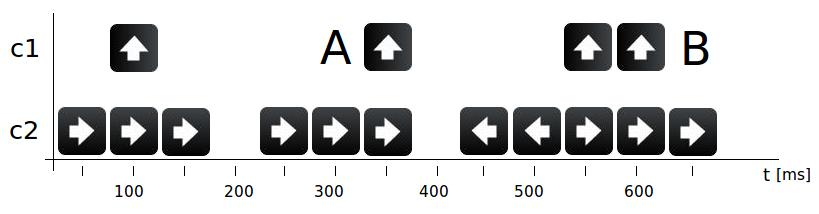
\includegraphics[width=\textwidth]{obrazki/sterowanie.jpg}
		\caption{Sterowanie względem czasu.}
		\label{fig:sterowanie}
		\end{figure}
		\end{par}
		
		Tablice c1, c2 oznaczają odpowiednio tablicę odpowiadającą za ruchy specjalne (np. skok), oraz tablicę odpowiadającą jedynie za ruch.

		Lepszym rozwiązaniem jest realizacja krzyżowania nie poprzez klasyczne podejście, lecz modelowane statystycznie: Potomstwo nie otrzymuje bezpośrednich fragmentów chromosomu, lecz losuje za każdym razem nowe ruchy. Przy czym chromosomy populacji rodzicielskiej zwiększają prawdopodobieństwo wylosowania podobnych sobie ruchów. Schemat takiego rozwiązania zaprezentowany jest na rysunku \ref{fig:krzyżowanie}. Więcej szczegółów na ten temat zostanie opisanych w dalszej części pracy.
		
		\begin{par}
		\begin{figure}[!h]
		\centering
		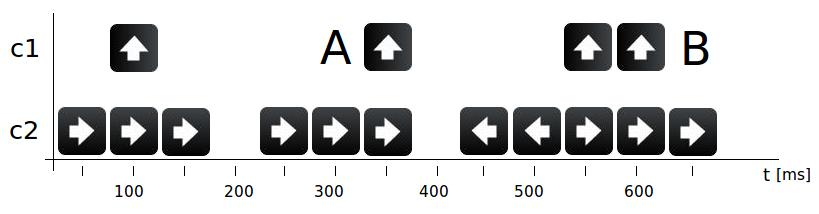
\includegraphics[width=\textwidth]{obrazki/sterowanie.jpg}
		\caption{Krzyżowanie statystyczne.}
		\label{fig:krzyżowanie}
		\end{figure}
		\end{par}

	\end{par}
	\item
	{\bf Aktualna pozycja gracza.}
	\begin{par}
		O ile poprzednie rozwiązanie dawało większą swobodę ruchu po mapie, to było jednak mało optymalne pod względem osiągania szybko dobrych wyników.
		Jeśli założymy iż akcje przechowywane w chromosomie mają być aktywowane w momencie osiągnięcia przez gracza danej pozycji na osi X mapy, wówczas uprościmy cały mechanizm krzyżowania (już nie musimy szukać punktów wspólnych, gdyż dwa dowolne indeksy w obu tablicach $i,j$ gwarantują nam takie samo położenie gracza na mapie gdy $i=j$.
		Oprócz tego przy założeniu że planszę da się rozwiązać poruszając się tylko w prawo upraszcza to większość operacji w algorytmie.
		Innym udogodnieniem będzie uproszczenie samego typu przechowywanych danych. Ponieważ rezygnujemy z postojów i ruchu w lewo, równie dobrze możemy zrezygnować z tablicy przechowującej te informacje.

		\begin{par}
		\begin{figure}[!h]
		\centering
		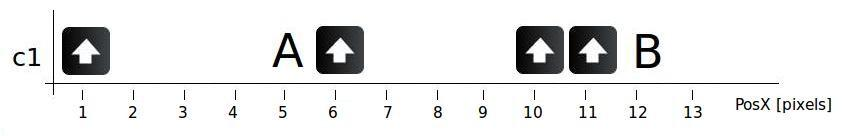
\includegraphics[width=\textwidth]{obrazki/sterowanie2.jpg}
		\caption{Sterowanie względem pozycji gracza.}
		\label{fig:sterowanie2}
		\end{figure}
		\end{par}

		To podejście posiada jednak kilka poważnych wad i wymaga pewnych ograniczajacych założeń.
		Plansza musi być ukierunkowana, i być rozwiązywalną przy ciągłym ruchu w określonym kierunku.
		Przeniesienie systemu do zastosowania w grze platformowej o nieco innym schemacie ruchu może okazać się trudne i wymagajace zmian w założeniach początkowych.
	\end{par}
	\end{enumerate}
\end{par}



\subsection{Diagram przypadków użycia}
\begin{par}
	Diagram przypadków użycia został przedstawiony na Rys. \ref{fig:diagram_przypadkow}.
		\begin{figure}[!h]
		\centering
		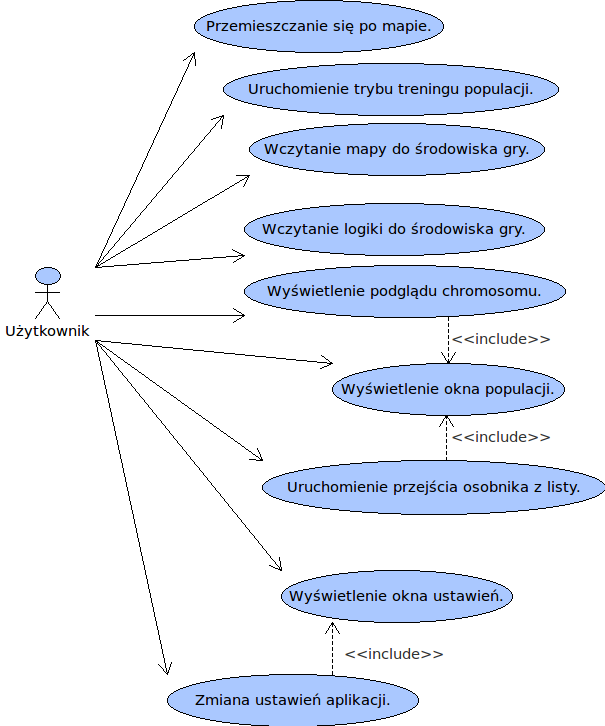
\includegraphics[width=\textwidth]{obrazki/diagram_przypadkow.png}
		\caption{Diagram przypadków użycia.}
		\label{fig:diagram_przypadkow}
		\end{figure}
\end{par}

\subsection{Diagram klas}
\begin{par}
	\begin{par}
	Diagram klas projektu przedstawiony został na rysunku \ref{fig:diagram_klas}.
	\end{par}
	\begin{figure}[!h]
	\centering
	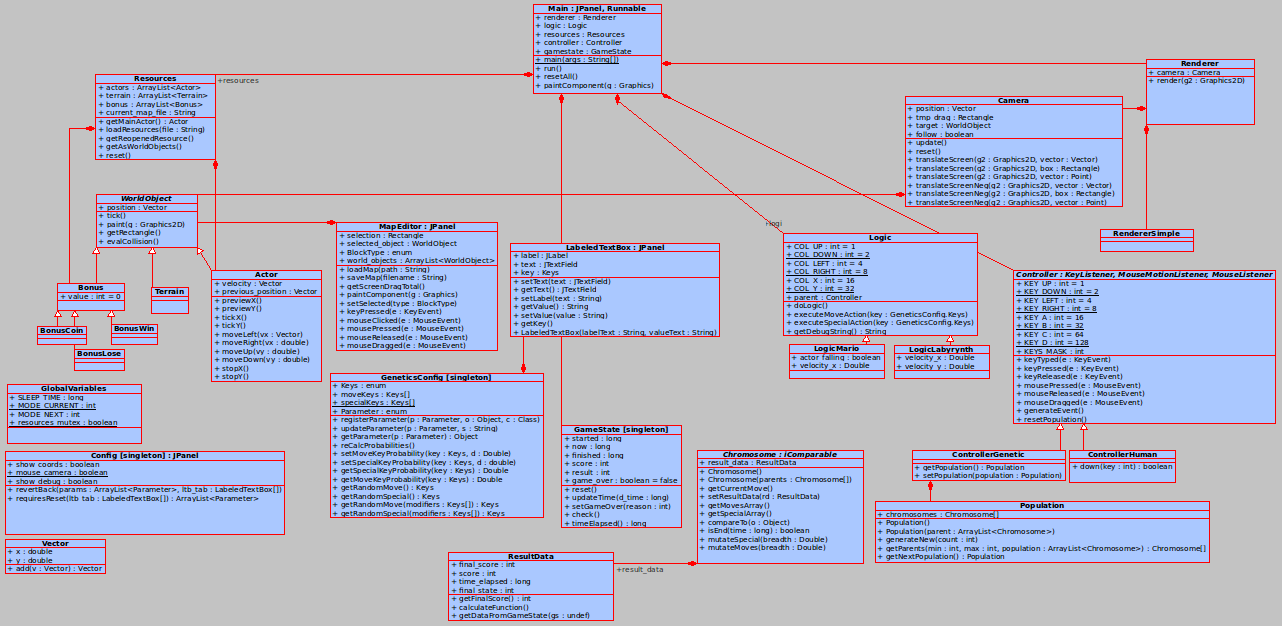
\includegraphics[width=\textwidth]{obrazki/diagram_klas.png}
	\caption{Diagram Klas.}
	\label{fig:diagram_klas}
	\end{figure}
\end{par}


